\documentclass[a4paper,12pt]{article}

\usepackage{amsmath,amssymb,amsthm,tikz}
\usetikzlibrary{calc,arrows.meta}
\usepackage[margin=20mm]{geometry}
\usepackage{fancyvrb}
\usepackage{enumerate}
\usepackage{hyperref}

\setlength{\parindent}{0pt}
\setlength{\columnsep}{1cm}

\begin{document}
\thispagestyle{empty}

\twocolumn

\begin{center}
{\Large Midterm. 2020-10-22},\\
{\em 100 minutes (9:00 \textendash{} 10:40)} 
\end{center}


%(1) Jau gatava C++ koda gabala analīze (tur ir cikli, 
%funkciju izsaukumi - jāatbild uz jautājumiem);
%arī jāuzraksta Big-O notation time complexity tam koda gabalam.
%(2) Objektorientēta C++ koda analīze (virtuālas funkcijas: 
%Jāpasaka, kura funkcija tiks izsaukta - vecāka klasē vai bērna klasē). 
%Ja kāds fiksi mācēs testēt kodu - varēs pārbaudīt uz sava kompilatora; 
%bet bez izpratnes cilvēki ar šo var kļūdīties.
%(3) Daži piemēri par Big-O notation - jāsalīdzina funkciju augšana.  
%(4) Stekam dots pseidokods, kur ar "push()" un "pop()" kaut ko dara; 
%jāuzraksta steka stāvokļi pēc komandu izpildes.
%(5) Uzdevums, kurā noteiktā veidā jāapstaigā pilns/complete koks, 
%kas dots ar masīvu (post-order, piemēram). Visnotaļ līdzīgs tam piemēram, 
%kuru atsūtīji - iespējams, mazliet vienkāršāks 
%(koks ir pilns - tātad tukšu vietu masīvā nemaz nav)



\vspace{10pt}
{\bf Question 1.} 

There is a 2-dimensional array $\mathtt{arr}$ 
of size $n$ by $n$; its elements are
integer numbers (each number contains no more than $n$ digits in 
its decimal representation). 

You are given this C++ code with function {\tt main()} calling function {\tt fun()}.
%On Line ? of this code we perform {\em integer division} (for example, $7/2$ equals $3$). 


{\footnotesize
\begin{center}
\begin{minipage}{.85\columnwidth}
\begin{Verbatim}[frame=single,numbers=left]
int fun(int row) {
  int count = 0;
  for (int col=0; col<n; col++) {
    while (arr[row][col]>0) {
      arr[row][col] /= 2;
      count++;
    }
  }
  return count;
}


int main() {
  for (int row=0; row<n; row++) {
    cout << fun(row);
  }
}
\end{Verbatim}
\end{minipage}
\end{center}
}

Analyze the time complexity of this algorithm 
``inside out'':

\begin{enumerate}[(A)]
\item Estimate with some $O(g(n))$ the time spent 
on a single iteration of the loop in 
Lines 5-6. (How fast one can run these lines
just once.)
\item Estimate with some $O(g(n))$ the time spent
on the loop Lines 4-7 (for one specific pair 
of row,col). 
\item Estimate with some $O(g(n))$ the 
time spent in the outer loop on Lines 3-8. 
(And also in a single call of {\tt fun(...)}.)
\item Estimate the time spent in the loop 
on Lines 14-16. 
\end{enumerate}


\textcolor{blue}{\footnotesize
{\em Note.} We use integer division in this algorithm; 
for example {\tt 7/2} equals {\tt 3} and {\tt 1/2} equals {\tt 0}. So it will eventually stop.
}






\vspace{20pt}
{\bf Question 2.} 

Definition of Big-O:\\
Real-valued function with natural arguments $f(n)$ is in 
$O(g(n))$ iff there exist $C,n_0 >0$ such that
$$|f(n)| \leq C \cdot |g(n)|,$$
whenever $n > n_0$. 

\begin{enumerate}[(A)]
\item Use the definition of Big-O Notation to 
prove or to disprove that $f(n) = 100n^2 + \frac{1}{4}n^3$
is in $O(n^3)$. 
\item Use the definition of Big-O Notation to 
prove or to disprove that $f(n) = (\log_2 n)^2$
is in $O(\log_2 n)$. 
\end{enumerate}

The reasoning should either provide the examples of $C,n_0$ 
that satisfy the definition for any $n$; or a method that 
for any given $C,n_0$ finds find $n$ such that the definition is not satisfied.




\vspace{20pt}
{\bf Question 3.} 

Consider the Queue implementation from \url{https://bit.ly/35n7bKd}.

Denote $a,b,c$ to be the last $3$ digits of your Student ID, and compute the following numbers: 
\begin{itemize}
\item $F = ((a+b+c)\;\operatorname{mod}\;3) + 2$
\item $\mathtt{x1} = (a+b+c)\;\operatorname{mod}\;10$
\item $\mathtt{x2} = ((a+b) \cdot 2)\;\operatorname{mod}\;10$
\item $\mathtt{x3} = ((b+c) \cdot 3)\;\operatorname{mod}\;10$
\item $\mathtt{x4} = ((c+a) \cdot 7)\;\operatorname{mod}\;10$
\end{itemize}

The queue $Q$ is implemented as an array of size $N=6$; its elements
have indices from $\{0,1,2,3,4,5\}$. 

Initially the queue parameters are these:\\
$\mathtt{Q.front} = \mathtt{F}$,\\
$\mathtt{Q.length} = 4$,\\
$\mathtt{Q.size} = 6$.\\
And the content of the array is the following:

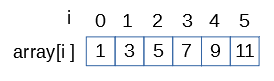
\includegraphics[width=2in]{midterm/midterm-queue-structure.png}

Somebody runs the following code on this queue:

\begin{verbatim}
Q.enqueue(x1)
Q.enqueue(x2)
Q.dequeue()
Q.dequeue()
// show the state of Q
Q.enqueue(x3)
Q.enqueue(x4)
Q.dequeue()
// show the state of Q
\end{verbatim}

After Line 4 (and at the very end) show the current state of the queue $\mathtt{Q}$. 
The state should display the content of the array and also the values of 
$\mathtt{Q.front}$ and $\mathtt{Q.length}$. 

You can use shading, if it helps to visualize the array cells that are not 
currently used by your queue.


\textcolor{blue}{\footnotesize
{\em Note.} Painting something gray is not required (since front/length indicate the state of your queue anyway). But painting cells gray may be helpful, if you want to visualize where your queue has the useful values (and what is some old garbage \textendash{} you can shade it over).
}


% https://www.geeksforgeeks.org/iterative-postorder-traversal-using-stack/
\vspace{20pt}
{\bf Question 4.} 

{\footnotesize
{\bf Introduction.} 
Binary trees are often represented as arrays 
(where the array starts with the root node; followed
by all the other nodes, displayed layer by layer. 
If any child of a node in this tree is missing, it is replaced by 
$\Lambda$ (capital Lambda denoting an empty tree)
in the array. Once we reach the last non-empty node in the tree, this is
the last element of the array. 
For example, the binary tree shown in this picture:

\begin{figure}[!htb]
\center{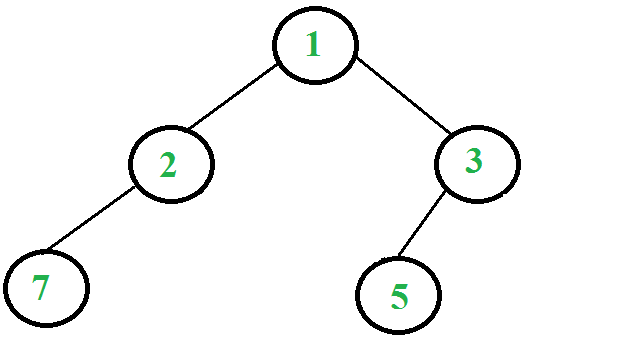
\includegraphics[width=2in]{midterm/example-binary-tree.png}}
\caption{\label{fig:example-binary-tree} Example binary tree.}
\end{figure}
is represented by the following array: 
$$\mathtt{int\;a[\,]\;=\;\{1,2,3,7,\Lambda,5\}};$$

}

\vspace{10pt}
{\bf Problem.} 
Assume that you have a binary tree that is represented by the following array:
\textcolor{red}{
\begin{equation}
\label{eq:treearr}
\mathtt{int\;a[\,]\;=\;\{1, 2, 4, a, \Lambda, \Lambda, 6, b, \Lambda, \Lambda, \Lambda, \Lambda, \Lambda, \Lambda, c\};}
\end{equation}
}

Values $a$, $b$, $c$ are the last three digits taken from your Student ID.\\
\textcolor{blue}{\footnotesize
{\em Note.} In the original the array contained a mistake (it had four $\Lambda$ 
instead of six; but this was wrong, it does not correspond to any tree). 
}


\begin{enumerate}[(A)]
\item Draw the binary tree represented by the array \ref{eq:treearr} in your answer. 
The tree should look nice: 
Draw left children to the left (and right children to the right)
of their parents. Nodes on the same levels should be aligned. 
\item What is the number of internal nodes in this tree? The number of leaves in this tree?
\item List the vertices of this tree in the post-order traversal order.\\
\textcolor{blue}{\footnotesize
{\em Note.} You only show real nodes in the post-order sequence (all $\Lambda$ are 
just technical symbols indicating absence of nodes; they are not part of the tree). 
}
\item Write pseudo-code for an algorithm\\ 
$\text{\textsc{getParent}}(i)$ that receives 
the index $i$ of some node in this array, returns the index of the parent of this node (or $-1$, if the node has no parent). 
All indices $i$ are zero-based (in an array of length $10$, $i \in \{0,\ldots,9\}$).
\item Assume that there is a different array (representing another binary tree) which does not contain any $\Lambda$ 
values; all values there represent some nodes. Describe the property such trees must satisfy.  
\end{enumerate}



\newpage

{\bf Question 1.} 

\begin{figure}[!htb]
\center{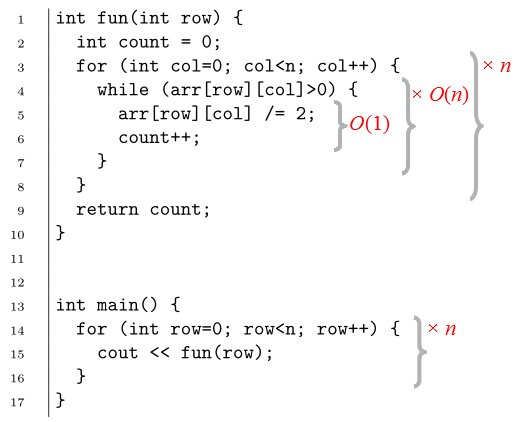
\includegraphics[width=3.5in]{midterm/prob3-pseudocode.png}}
\caption{\label{fig:prob3-pseudocode} Time complexity (inside out).}
\end{figure}

To estimate time complexity from the given code or pseudocode, 
you can work inside out (first estimate the time complexity for 
a single loop iteration, then estimate how many times the loop itself is executed, 
then multiply both estimates, etc.). 


{\bf (A)} Lines 5--6.\\ 
Time is $O(1)$, since these are 
just two operations on 4-byte integers. 
(It is obviously true for the regular {\tt int} type. 
Even in the case when $n$ is very large number and the
array elements do not fit into the 4-byte register, 
division by $2$ can take constant time, if number is 
written into binary notation: it is just the right shift.)

{\bf (B)} Lines 4--7.\\
Time is $O(n) \cdot O(1) = O(n)$.\\
To verify this claim, note that 
any array element is a number with $n$ digits 
(in decimal notation).
Its value is at most $10^n$. 
In order to have $k$ iterations of the {\bf while} 
loop (before {\tt arr[row][col]} turns to $0$) we should
have $10^n \geq 2^k$, i.e. $k \leq n \cdot \log_2 10$ is in $O(n)$.

{\bf (C)} Lines 3--8.\\
Time is $n \cdot  O(n) = O(n^2)$.\\
Indeed, the for-loop (Line 3) executes $n$ times; 
so we multiply $n$ by $O(n)$ and get $O(n^2)$.

{\bf (D)} Lines 14--16.\\
Time is $O(n) \cdot O(n \cdot n) = O(n^3)$. 
Method {\tt main()} calls function {\tt fun} 
$n$ times.


\vspace{20pt}
{\bf Question 2.}\\
{\bf (A)} Answer: True.\\
We prove that $f(n) = 100n^2 + \frac{1}{4}n^3$ 
is in $O(n^3)$.\\
{\em Proof.} Select $n_0 = 1$, $C = 100\frac{1}{4}$.
Denote $g(n) = n^3$. We check that $f(n)$ is in $O(g(n))$. 

For each $n \geq n_0 =1$ we have $n^2 \leq n^3$ and therefore
$$|f(n)| = |100n^2 + \frac{1}{4}n^3| \leq |100n^3 + \frac{1}{4}n^3| =$$
$$= |100\frac{1}{4}n^3| \leq 101\frac{1}{4}|n^3| = C \cdot |g(n)|.$$


{\bf (B)} Answer: False.\\
We state that $f(n) = (\log_2 n)^2$
is not in $O(g(n))$, where we denote $g(n) = \log_2 n$. 

Assume from contrary that somebody has selected $n_0$ and $C$ such 
that for every $n \geq n_0$ we have:
$$|f(n)| \leq C |g(n)|.$$
We pick $n$ such that $\log_2 n > C$ or $n > 2^C$ and simultaneosly 
$n \geq n_0$ (we can have the maximum of both $2^C$ and $n_0$). 

{\em Note.} This example can also demonstrate, why 
it is not easy to estimate the Big-O notation from computer-generated
function graphs. If you pick, say $C = 100$, 
the values $n$ where $|f(n)|$ exceeds $C|g(n)|$ 
may become quite large. 

\begin{figure}[!htb]
\center{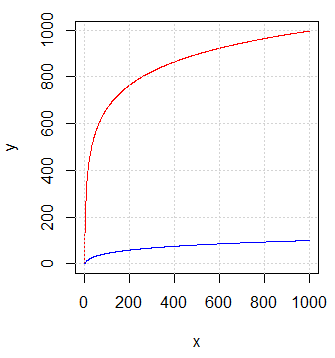
\includegraphics[width=3.2in]{midterm/solution-log-log-graph.png}}
\caption{\label{fig:solution-log-log-graph} Insufficient interval for $x$.}
\end{figure}


See Figure~\ref{fig:solution-log-log-graph}.
It seems that the red graph $y = 100 \cdot g(x) = 100 \cdot \log_2 x$ 
is much larger than the blue graph $y = f(x) = (\log_2 x)^2$. 
The problem with these graphs is the very short interval 
$x \in [1;1000]$ where these functions 
are compared. 

If you consider $x \in \left[ 1; 5\cdot 10^{30} \right]$, it
is easy to see that the logarithm squared (the blue function $f(x)$) 
overtakes the red function $100 \cdot g(x) = 100 \cdot \log_2 x$.
See Figure~\ref{fig:solution-log-log-graph2}.
In practice it is much better to use 
limit calculus (because with function graphs it is hard to tell, how 
far you need to draw before you can see which expression is bigger):
$$\lim_{x \rightarrow \infty} \frac{(\log_2 x)^2}{\log_2 x} =
\lim_{x \rightarrow \infty} \log_2 x = +\infty.$$


\begin{figure}[!htb]
\center{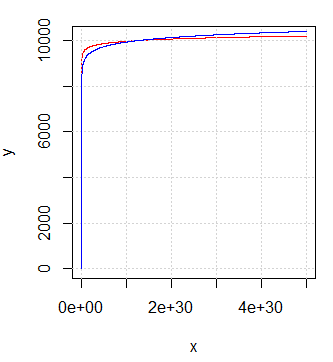
\includegraphics[width=3.2in]{midterm/solution-log-log-graph2.png}}
\caption{\label{fig:solution-log-log-graph2} 
${\displaystyle g(x) = \left(\log_2 x\right)^2}$ not in $O(\log_2 x)$.}
\end{figure}




\vspace{20pt}
{\bf Question 3.} Let us show queue after each queue operation. 
Let us consider one particular example. for your $a,b,c$ the
result may look different; it might be ``rotated'', because
$F$ (the front pointer) is different. Also the newly enqueued
values ($x_1, \ldots$) will likely be different. Your queue 
will also have $4$ entries (unshaded cells) at the start 
and $5$ entries at the very end.

We take $abc = 789$. For these values we have these initial values:
{\footnotesize
$$F = 2,\;\;L = 4,\;\;x_1 = 4,\;\;x_2 = 0,\;\;x_3 = 1,\;\;x_4 = 2.$$
}


\begin{figure}[!htb]
\center{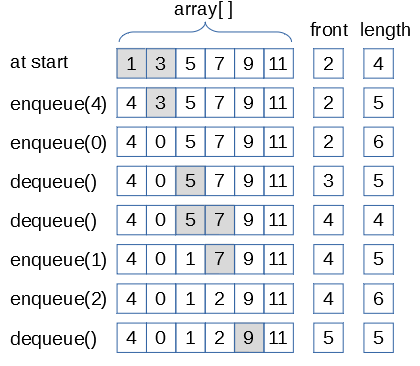
\includegraphics[width=3in]{midterm/solution-prob3.png}}
\caption{\label{fig:solution-prob3} Queue states.}
\end{figure}


\vspace{20pt}
{\bf Question 4.}\\
{\bf (A)} The array and corresponding tree are shown below: 
$$\mathtt{int\;a[\,]\;=\;\{1, 2, 4, a, \Lambda, \Lambda, 6, b, \Lambda, \Lambda, \Lambda, \Lambda, \Lambda, \Lambda, c\};}$$

\begin{figure}[!htb]
\center{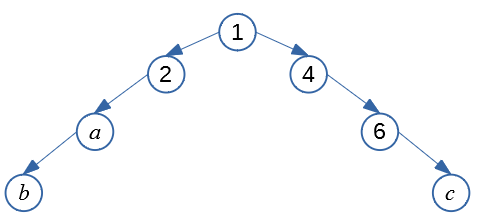
\includegraphics[width=3in]{midterm/prob4-binary-tree.png}}
\caption{\label{fig:prob4-midterm-binary-tree} Binary tree for the array.}
\end{figure}

\vspace{5pt}
{\bf (B)} There are $5$ internal nodes and $2$ leaves. 

\vspace{5pt}
{\bf (C)} Postorder sequence for the nodes (namely, first visit both subtrees in postorder, then the parent)
is the following: 
$$b,a,2,c,6,4,1.$$

\vspace{5pt}
{\bf (D)} The pseudocode is given below:
\[
\begin{array}{rl}
 & \text{\sc getParent}(i)\\
1 & \text{\textbf{if\ }}i\;\text{mod}\;2 ==0:\\
2 & \hspace{.5cm} \text{\textbf{return\ }} (i-2)/2\\
3 & \text{\textbf{if\ }}i\;\text{mod}\;2 ==1:\\
4 & \hspace{.5cm} \text{\textbf{return\ }} (i-1)/2\\
\end{array}
\]
You can also merge both formulas and get this formula:
$$\text{\sc getParent}(i) = \left\lfloor \frac{i-1}{2} \right\rfloor.$$
Here we use the floor function (rounding down). 

\vspace{5pt}
{\bf (E)} Such trees are called {\em complete trees} (all levels in such trees are full, 
except maybe the last level, which can be only partially full, but is filled
without any interruptions from the left side). 








\end{document}



